\chapter{Project Design and Implementation}

\section{Proposed Project Architecture}

The system is organized as a layered pipeline in which each layer consumes a well-defined data structure from the layer above it and produces one for the layer below. The layering is the direct consequence of the requirement that every optimization pass be independent and reorderable: if a pass could reach into the parser, or the code generator could depend on which passes had run, ordering experiments would be confounded by hidden coupling. Every boundary in \fig{fig:architecture} is therefore a plain Python data structure, a list of tokens, a syntax tree, a list of instructions, or a metrics record, and no layer holds a reference to any other layer's internal state.

\begin{figure}[!htb]
\centering
\resizebox{\textwidth}{!}{%
\begin{tikzpicture}[
  font=\footnotesize,
  layer/.style={draw=black!35, rounded corners=3pt, inner sep=6pt, fill=#1},
  comp/.style={draw, rounded corners=2pt, fill=white, minimum height=0.85cm, minimum width=2.35cm, align=center, font=\footnotesize},
  data/.style={font=\scriptsize\itshape, text=black!65},
  arr/.style={-{Stealth[length=2.2mm]}, thick, black!70},
  lbl/.style={font=\scriptsize\bfseries, text=black!70, anchor=west}]

% Presentation layer
\node[comp] (cli) at (0,0) {Command-line\\driver};
\node[comp, right=6mm of cli] (api) {FastAPI\\JSON API};
\node[comp, right=6mm of api] (react) {React\\web app};
\node[comp, right=6mm of react] (legacy) {Legacy\\HTML page};
\begin{scope}[on background layer]
\node[layer=blue!6, fit=(cli)(legacy), label={[lbl]above left:Presentation layer}] (L6) {};
\end{scope}
\draw[arr] (react) -- (api);
\draw[arr] (legacy) -- (api);

% Measurement layer
\node[comp, below=14mm of cli] (metrics) {Metric\\collector};
\node[comp, right=6mm of metrics] (viz) {Visualizer\\(7 plot types)};
\node[comp, right=6mm of viz] (geo) {Geometric-mean\\summary};
\begin{scope}[on background layer]
\node[layer=green!6, fit=(metrics)(geo), label={[lbl]above left:Measurement layer}] (L5) {};
\end{scope}

% Execution / backend layer
\node[comp, below=14mm of metrics] (interp) {IR interpreter\\(dynamic count, output)};
\node[comp, right=6mm of interp] (codegen) {RISC-V RV32IM\\code generator};
\node[comp, right=6mm of codegen] (sim) {RV32IM simulator\\(test oracle)};
\begin{scope}[on background layer]
\node[layer=orange!7, fit=(interp)(sim), label={[lbl]above left:Execution and back-end layer}] (L4) {};
\end{scope}
\draw[arr] (codegen) -- (sim);

% Optimization layer
\node[comp, below=14mm of interp] (pm) {Pass manager\\(orderings, permutations)};
\node[comp, right=6mm of pm, minimum width=5.1cm] (passes) {Six passes: CF, DCE, CSE, CP, SR, AS\\each: list[IRInstruction] $\to$ list[IRInstruction]};
\begin{scope}[on background layer]
\node[layer=violet!6, fit=(pm)(passes), label={[lbl]above left:Optimization layer}] (L3) {};
\end{scope}
\draw[arr] (pm) -- (passes);

% Middle layer
\node[comp, below=14mm of pm] (irgen) {IR generator};
\node[comp, right=6mm of irgen] (ir) {Three-address code\\(35 opcodes)};
\node[comp, right=6mm of ir] (symtab) {Symbol table\\(scope stack)};
\begin{scope}[on background layer]
\node[layer=yellow!10, fit=(irgen)(symtab), label={[lbl]above left:Intermediate representation layer}] (L2) {};
\end{scope}
\draw[arr] (symtab) -- (irgen);

% Front end
\node[comp, below=14mm of irgen] (lexer) {Lexer};
\node[comp, right=6mm of lexer] (parser) {Recursive-descent\\parser};
\node[comp, right=6mm of parser] (ast) {AST\\(20 node types)};
\node[comp, right=6mm of ast] (sema) {Semantic\\analyzer};
\begin{scope}[on background layer]
\node[layer=red!5, fit=(lexer)(sema), label={[lbl]above left:Front-end layer}] (L1) {};
\end{scope}
\draw[arr] (lexer) -- node[data, above]{tokens} (parser);
\draw[arr] (parser) -- node[data, above]{tree} (ast);
\draw[arr] (ast) -- (sema);

% Source
\node[comp, below=12mm of lexer, fill=gray!10] (src) {C-subset source\\(15 benchmarks, user code)};
\draw[arr] (src) -- (lexer);

% Vertical flows between layers
\draw[arr] (ast.north) -- ++(0,0.55) -| node[data, pos=0.25, above]{validated AST} (irgen.south);
\draw[arr] (ir.north) -- node[data, right]{baseline IR} (passes.south);
\draw[arr] (passes.north) -- node[data, right]{optimized IR} (codegen.south);
\draw[arr] (pm.north) -- node[data, right]{optimized IR} (interp.south);
\draw[arr] (interp.north) -- node[data, right]{dynamic metrics} (metrics.south);
\draw[arr] (metrics.north) -- node[data, right]{metrics} (cli.south);
\draw[arr] (geo.north) -- node[data, right]{summary} (react.south);
\end{tikzpicture}}
\caption[Layered architecture of the compiler infrastructure.]{Layered architecture of the compiler infrastructure. Every arrow carries a plain data structure; no layer depends on the internal state of another. The optimization layer is the subject of the study and is the only layer whose behaviour changes between experiments.}
\label{fig:architecture}
\end{figure}

\textbf{Front-end layer.} The front end turns source text into a validated abstract syntax tree. The lexer produces tokens with line and column positions. The recursive-descent parser produces the tree. The semantic analyzer walks the tree with its own scope stack, checks every rule that the grammar cannot express, and collects all violations. Only a tree that passes semantic analysis reaches the next layer, which means every later component may assume that names resolve, arities match, and arrays are used as arrays.

\textbf{Intermediate representation layer.} The IR generator walks the validated tree and emits a flat list of three-address instructions, allocating temporaries \code{t0}, \code{t1}, \ldots{} and labels \code{L0}, \code{L1}, \ldots{} as it goes, and consulting a scope-aware symbol table to map source names to unique IR names when shadowing occurs. The instruction list is the central data structure of the whole system: every optimization pass, the interpreter, the metric collector, and the code generator operate on it and nothing else.

\textbf{Optimization layer.} This is the layer under study. Six passes are registered by short name in a dictionary. The pass manager accepts an ordered list of names, validates it against the registry, and folds the IR through the passes in that order, copying the list first so that the baseline is never mutated. It also enumerates all full permutations of the registry. Each pass is a pure function; passes share no state and communicate only through the instruction list.

\textbf{Execution and back-end layer.} Two consumers of the optimized IR live here. The interpreter executes the IR directly, producing program output, a dynamic instruction count, and per-opcode frequencies; it is the oracle for correctness, since an ordering is accepted only if its output equals the baseline's. The RISC-V code generator lowers the IR to RV32IM assembly, and a small simulator executes that assembly in tests to confirm that lowering preserves behaviour.

\textbf{Measurement layer.} The metric collector computes static code size, an estimated cycle cost from a cost table, and an instruction-category breakdown for any instruction list, and combines them with the interpreter's dynamic results into a single record per ordering. The visualizer renders records into plots, and the summary module computes geometric means across programs.

\textbf{Presentation layer.} The command-line driver and the FastAPI server are two thin front doors to the same modules. The server exposes seven JSON endpoints and serves the pre-built React application; the legacy single-file page from Phase I remains available at a secondary route. Neither front door contains compiler logic.

\section{High Level Design}

Two workflows run through the architecture: the exhaustive benchmark experiment, which is a batch process driven from the command line, and the interactive session, which is a request-response process driven from the browser.

\begin{figure}[!htb]
\centering
\resizebox{\textwidth}{!}{%
\begin{tikzpicture}[
  font=\footnotesize, node distance=5mm and 8mm,
  stp/.style={draw, rounded corners=2pt, fill=white, minimum height=0.8cm, minimum width=2.6cm, align=center},
  loop/.style={draw=black!40, dashed, rounded corners=4pt, inner sep=7pt},
  arr/.style={-{Stealth[length=2.2mm]}, thick, black!70},
  d/.style={font=\scriptsize\itshape, text=black!65}]
\node[stp] (s1) {benchmark\\program (.c)};
\node[stp, right=of s1] (s2) {lex, parse,\\check, generate};
\node[stp, right=of s2] (s3) {baseline IR};
\node[stp, right=of s3] (s4) {interpret baseline\\(reference output)};
\draw[arr] (s1) -- (s2); \draw[arr] (s2) -- (s3); \draw[arr] (s3) -- (s4);

\node[stp, below=14mm of s2] (l1) {ordering $\sigma$\\(1 of 721)};
\node[stp, right=of l1] (l2) {pass manager\\runs $\sigma$ on IR};
\node[stp, right=of l2] (l3) {interpret result;\\compare output};
\node[stp, right=of l3] (l4) {collect static and\\dynamic metrics};
\draw[arr] (l1) -- (l2); \draw[arr] (l2) -- (l3); \draw[arr] (l3) -- (l4);
\draw[arr] (s3.south) -- ++(0,-0.4) -| (l2.north);
\draw[arr] (s4.south) -- ++(0,-0.4) -| node[d, pos=0.75, right]{expected output} (l3.north);
\begin{scope}[on background layer]
\node[loop, fit=(l1)(l4), label={[font=\scriptsize\bfseries, text=black!60]below left:for each of the 720 permutations and the empty ordering}] {};
\end{scope}

\node[stp, below=16mm of l2] (r1) {721 metric\\records};
\node[stp, right=of r1] (r2) {per-program plots\\(6 per program)};
\node[stp, right=of r2] (r3) {cross-program box\\plot, geomean table};
\draw[arr] (l4.south) -- ++(0,-0.45) -| (r1.north);
\draw[arr] (r1) -- (r2); \draw[arr] (r2) -- (r3);
\node[d, below=1mm of r3] {repeated for all 15 programs};
\end{tikzpicture}}
\caption[High-level design of the exhaustive benchmark workflow.]{High-level design of the exhaustive benchmark workflow. The baseline IR is generated once per program and every ordering is applied to a copy of it. Each result is interpreted and its output compared with the baseline before its metrics are trusted.}
\label{fig:hld-benchmark}
\end{figure}

\textbf{Benchmark workflow.} For each of the fifteen programs, the driver reads the source, runs the front end once to obtain the baseline IR, and interprets the baseline to obtain the reference output. It then iterates over the 721 orderings. For each, it runs the pass manager on a copy of the baseline IR, interprets the optimized IR to obtain the dynamic instruction count, opcode frequencies, and output, compares the output with the reference, and hands the optimized IR and the dynamic results to the metric collector, which returns one record containing the ordering, its label, the static code size, the estimated cycles, the instruction breakdown, the dynamic count, and a correctness flag. After all orderings have been processed the visualizer produces six plots for the program; after all programs, it produces the cross-program box plot and the geometric-mean table, and the driver prints the best ordering per program and warns if any ordering anywhere produced incorrect output. The whole run takes about 24 seconds on the reference machine.

\begin{figure}[!htb]
\centering
\resizebox{\textwidth}{!}{%
\begin{tikzpicture}[
  font=\footnotesize, node distance=4mm and 10mm,
  box/.style={draw, rounded corners=2pt, fill=white, minimum height=0.75cm, minimum width=3.0cm, align=center},
  ep/.style={draw, rounded corners=2pt, fill=blue!5, minimum height=0.62cm, minimum width=3.4cm, align=left, font=\scriptsize\ttfamily},
  arr/.style={-{Stealth[length=2.2mm]}, thick, black!70},
  grp/.style={draw=black!35, rounded corners=3pt, inner sep=6pt}]
\node[box] (pg) {Playground};
\node[box, below=of pg] (ol) {Optimization Lab};
\node[box, below=of ol] (as) {Assembly};
\node[box, below=of as] (ex) {Phase Explorer};
\node[box, below=of ex] (rf) {Reference};
\begin{scope}[on background layer]
\node[grp, fit=(pg)(rf), label={[font=\scriptsize\bfseries]above:React front end (browser)}] (FE) {};
\end{scope}

\node[ep, right=22mm of pg] (e1) {POST /api/compile};
\node[ep, below=of e1] (e2) {POST /api/optimize-steps};
\node[ep, below=of e2] (e3) {POST /api/assembly};
\node[ep, below=of e3] (e4) {POST /api/benchmark};
\node[ep, below=of e4] (e5) {GET /api/examples[/\{name\}]};
\node[ep, below=of e5] (e6) {POST /api/optimize};
\begin{scope}[on background layer]
\node[grp, fit=(e1)(e6), label={[font=\scriptsize\bfseries]above:FastAPI server (JSON over HTTP)}] (BE) {};
\end{scope}

\node[box, right=20mm of e1, minimum width=3.2cm] (m1) {Lexer, Parser,\\Semantic analyzer};
\node[box, below=of m1, minimum width=3.2cm] (m2) {IR generator};
\node[box, below=of m2, minimum width=3.2cm] (m3) {Pass manager,\\six passes};
\node[box, below=of m3, minimum width=3.2cm] (m4) {Interpreter};
\node[box, below=of m4, minimum width=3.2cm] (m5) {RISC-V code generator};
\node[box, below=of m5, minimum width=3.2cm] (m6) {Metric collector};
\begin{scope}[on background layer]
\node[grp, fit=(m1)(m6), label={[font=\scriptsize\bfseries]above:Compiler modules (unchanged)}] (CM) {};
\end{scope}

\draw[arr] (pg) -- (e1);
\draw[arr] (ol) -- (e2);
\draw[arr] (as) -- (e3);
\draw[arr] (ex) -- (e4);
\draw[arr] (FE.east |- e5) -- (e5);
\draw[arr] (BE.east |- m1) -- (m1);
\draw[arr] (BE.east |- m3) -- (m3);
\draw[arr] (BE.east |- m4) -- (m4);
\draw[arr] (BE.east |- m5) -- (m5);
\draw[arr] (BE.east |- m6) -- (m6);
\end{tikzpicture}}
\caption[High-level design of the interactive web application.]{High-level design of the interactive web application. Each page of the single-page React application calls one primary endpoint; the endpoints are thin adapters that call the same compiler modules the command-line driver uses and serialize the results to JSON.}
\label{fig:hld-web}
\end{figure}

\textbf{Interactive workflow.} The browser loads the React application from the FastAPI server. Each page issues JSON requests to one or two endpoints. The Playground calls \code{/api/compile}, which runs the front end and IR generator and returns tokens, a serialized syntax tree, the symbol list, and the IR both as structured records and as text; on failure it returns a structured error with the phase, message, line, and column, which the editor uses to underline the offending source. The Optimization Lab calls \code{/api/optimize-steps}, which applies the user's ordering one pass at a time and returns, for every stage, the IR text, a line diff against the previous stage, and the metrics. The Assembly page calls \code{/api/assembly}, which returns IR lines, assembly lines, and a mapping between them for hover linking. The Phase Explorer calls \code{/api/benchmark}, which runs all 721 orderings and returns their metrics for plotting in the browser. All pages share the example picker, which lists the fifteen benchmarks grouped by suite through \code{/api/examples}. Because the endpoints call the same modules as the command-line driver, any result seen in the browser is reproducible from the command line.

\section{Detailed Design}

This section describes each component in the order in which data flows through the system. Line counts are given to convey the scale of each module; the complete compiler core is about 4{,}000 lines of Python, the web layer about 1{,}200, the tests about 2{,}000, and the React front end about 1{,}900 lines of TypeScript and CSS.

\subsection{Lexer}

The lexer (\code{compiler/lexer.py}, 268 lines) is a hand-written scanner over the source string. It maintains a position, a line, and a column, and exposes a generator that yields tokens on demand. Each token is an immutable record with a type, the matched text, and the line and column where it began. There are 33 token types: two for literals and identifiers, seven keywords (\code{int}, \code{if}, \code{else}, \code{while}, \code{for}, \code{return}, \code{print}), five arithmetic operators, six comparison operators, three logical operators, assignment, eight delimiters, and an end-of-file marker. Two-character operators are recognized before one-character operators so that \code{<=} is never read as \code{<} followed by \code{=}. Both comment styles are skipped; an unterminated block comment and a digit sequence followed immediately by a letter are reported as lexical errors with the location of the offending construct. The lexer has no knowledge of the grammar and can be run and inspected independently, which the Playground's Tokens tab uses.

\subsection{Parser and abstract syntax tree}

The parser (\code{compiler/parser.py}, 444 lines) is a recursive-descent parser with one method per grammar production. The full grammar is given in Appendix~A. At the top level, a declaration whose third token is a left parenthesis is a function; otherwise it is a global variable. Inside a block, the first token of a statement selects the production: \code{int} for a declaration, which becomes an array declaration if a bracket follows the name; \code{if}, \code{while}, \code{for}, \code{return}, \code{print} for the corresponding statements; a brace for a nested block; and anything else for an assignment or expression statement, which is parsed as an expression and then reinterpreted as an assignment if an \code{=} follows, with the parsed expression required to be an identifier or an array access. An \code{else} followed by \code{if} wraps the nested conditional in an implicit block, giving \code{else if} chains without a dedicated grammar rule. The \code{for} statement allows any of its three clauses to be empty, and its initializer may be a declaration whose scope is the loop.

Expressions are parsed by precedence climbing through six levels: logical or, logical and, equality, comparison, additive, multiplicative, then unary minus and not, then primary expressions, which are integer literals, identifiers, function calls, array accesses, and parenthesized expressions. Every parse error raises an exception carrying the message, the expected construct, and the token actually found, so that a message such as ``Expected RPAREN after if condition (got SEMICOLON `;')'' with a line and column is produced.

The syntax tree (\code{compiler/ast\_nodes.py}, 173 lines) consists of twenty node types defined as Python dataclasses, all carrying a line and column: eight expression nodes (literal, identifier, binary, unary, call, assignment, array access, array assignment), nine statement nodes (variable declaration, array declaration, expression statement, block, if, while, for, return, print), and three top-level nodes (parameter, function declaration, program). The uniform dataclass representation allows the web layer to serialize any tree generically: each node becomes its type name, its scalar fields, and its child nodes in source order.

\subsection{Symbol table and semantic analyzer}

The symbol table (\code{compiler/symbol\_table.py}, 111 lines) is a stack of dictionaries, one per scope. Declaring a name that already exists in the innermost scope is an error; declaring a name that exists in an outer scope is shadowing, and the table assigns the inner variable a unique IR name by appending a counter, so that the flat IR can hold both variables without conflict. Each symbol records its kind (\code{int}, \code{array}, or \code{global}), its scope depth, its IR name, and, for arrays, its element count.

The semantic analyzer (\code{compiler/semantic\_analyzer.py}, 271 lines) runs between parsing and IR generation and enforces the rules listed in Table~\ref{tab:semantic-rules}. It first collects every function's name and arity so that calls may precede definitions, then walks each global and each function body with its own scope stack. Unlike the symbol table, which raises on the first error, the analyzer appends every violation to a list and raises a single exception carrying all of them at the end, so a user sees every problem in one compile. It was added in Phase II after the team observed that Phase I reported such errors from inside IR generation, one at a time and without source positions.

\begin{table}[!htb]
\centering\small
\caption[Rules enforced by the semantic analyzer.]{Rules enforced by the semantic analyzer}
\label{tab:semantic-rules}
\begin{tabular}{L{4.6cm} L{8.6cm}}
\toprule
\textbf{Rule} & \textbf{Reported as}\\
\midrule
Variable declared before use & Undeclared variable `x'\\
No duplicate name in one scope & Variable `x' already declared in this scope\\
Called function exists & Call to undefined function `f'\\
Argument count matches arity & Function `f' expects 2 arguments, got 3\\
No duplicate function definition & Function `f' is defined more than once\\
A \code{main} function exists & No main() function defined\\
Arrays are indexed, scalars are not & `a' is not an array; Array `a' cannot be used as a value\\
Array not assigned without index & Cannot assign to array `a' without an index\\
Global initializer is constant & Global `g' initializer must be a constant expression\\
Global does not shadow a function & Global `f' conflicts with a function of the same name\\
\bottomrule
\end{tabular}
\end{table}

\subsection{Intermediate representation}

The IR (\code{compiler/ir.py}, 253 lines) is a linear three-address code. Each instruction is a record with an opcode and up to three operand strings: a destination and two sources. Operands are variable names, temporary names, label names, or integer literals, and a helper distinguishes literals from names so that passes can treat constants uniformly. The 35 opcodes fall into eight groups, summarized in Table~\ref{tab:opcodes}; the complete reference is in Appendix~B.

\begin{table}[!htb]
\centering\small
\caption[Opcode groups of the three-address code.]{Opcode groups of the three-address code}
\label{tab:opcodes}
\begin{tabular}{L{3.2cm} L{6.0cm} L{3.9cm}}
\toprule
\textbf{Group} & \textbf{Opcodes} & \textbf{Form}\\
\midrule
Arithmetic & ADD, SUB, MUL, DIV, MOD, NEG & \code{d = a op b}, \code{d = -a}\\
Comparison & EQ, NEQ, LT, GT, LTE, GTE & \code{d = a cmp b} (0 or 1)\\
Logical & AND, OR, NOT & \code{d = a \&\& b}, \code{d = !a}\\
Data movement & COPY, LOAD\_CONST & \code{d = a}, \code{d = 5}\\
Control flow & LABEL, JUMP, JUMP\_IF\_TRUE, JUMP\_IF\_FALSE & \code{L:}, \code{goto L}, \code{if a goto L}\\
Functions & PARAM, CALL, RETURN, FUNC\_BEGIN, FUNC\_END, FUNC\_PARAM & \code{param a}, \code{d = call f, n}\\
Memory & ARR\_DECL, ARR\_LOAD, ARR\_STORE, GLOBAL\_DECL, GLOBAL\_LOAD, GLOBAL\_STORE & \code{d = a[i]}, \code{a[i] = v}, \code{d = @g}\\
Other & PRINT, NOP & \code{print a}\\
\bottomrule
\end{tabular}
\end{table}

Two design decisions in the IR are central to the safety of reordering. First, each instruction knows its own \emph{def} and \emph{use} sets: a method returns the variable the instruction writes, if any, and another returns the set of variables it reads, excluding literals. Every pass is written in terms of these two methods rather than in terms of opcodes, so adding an opcode requires updating only these methods for the passes to handle it correctly. Second, memory that outlives a basic block, arrays and global variables, is accessed only through dedicated opcodes. An array store is not a definition of any variable in the def-use sense and a global store is not either, so the local, block-scoped analyses used by the passes can never conclude that such a store is dead or that a value loaded from memory is still available after an intervening store. This is deliberately conservative; it trades some missed optimizations for the guarantee that the passes are correct without alias analysis.

\subsection{IR generator}

The IR generator (\code{compiler/ir\_generator.py}, 352 lines) walks the validated tree and emits instructions. Expressions return the name of the temporary or variable holding their value; literals are materialized with LOAD\_CONST, identifiers return their IR name directly (or a fresh temporary loaded from the global), binary operators emit one instruction into a fresh temporary, and calls emit one PARAM per argument followed by CALL. Control flow is lowered to labels and jumps in the standard way, as shown in Listing~\ref{lst:lowering}. Short-circuit operators are lowered to jumping code: the right operand is evaluated only when the left does not decide the result, and the result is normalized to 0 or 1 with a comparison against zero so that it agrees with the eager AND and OR opcodes. Functions are bracketed by FUNC\_BEGIN and FUNC\_END with one FUNC\_PARAM per parameter, and every variable declared without an initializer is set to zero, matching the zero-initialization of arrays.

\begin{lstlisting}[language=ThreeAC, caption={Lowering patterns used by the IR generator. Left: a while loop. Right: the short-circuit lowering of \code{a \&\& b}, in which \code{b} is evaluated only if \code{a} is true.}, label={lst:lowering}]
while (cond) { body }        |    r = a && b
                              |
L0:                           |      <code for a into ta>
  <code for cond into tc>     |      iffalse ta goto L2
  iffalse tc goto L1          |      <code for b into tb>
  <code for body>             |      r = tb != 0
  goto L0                     |      goto L3
L1:                           |    L2:
                              |      r = 0
                              |    L3:
\end{lstlisting}

\subsection{Interpreter}

The interpreter (\code{compiler/interpreter.py}, 307 lines) executes the IR directly. It indexes labels and function entry points once, then runs \code{main}. Each function call saves the caller's variables and arrays, binds arguments to the callee's FUNC\_PARAM slots, executes until RETURN or FUNC\_END, and restores the caller. Arguments are accumulated from PARAM instructions into a pending list consumed by the next CALL. Arithmetic uses Python integers; division and modulo by zero yield zero rather than raising, and array accesses outside bounds read zero and ignore writes, so that no valid program can crash the interpreter. Every instruction executed, including labels, increments a step counter and a per-opcode frequency table, and a limit of ten million steps guards against non-terminating input. The result record carries the return value, the list of printed integers, the step count, the frequency table, and whether the limit was reached. The step count is the project's dynamic instruction metric, and the printed output is the correctness oracle.

\subsection{Optimization passes}

Each pass lives in its own module under \code{compiler/optimizations/} and exports one function that takes an instruction list and returns a new one. None of them mutate their input. All six are local: they walk the list once (or to a fixed point) and reset any accumulated knowledge at every LABEL, JUMP, conditional jump, CALL, FUNC\_BEGIN, and FUNC\_END, because a value known before a label may be different when control arrives at the label from elsewhere. This is the classical basic-block restriction. It makes the passes weaker than their global counterparts, but it also makes their correctness independent of what ran before them, which is the property that permits arbitrary reordering.

\textbf{Constant folding (CF, 197 lines).} The pass first counts how many times each variable is defined. A variable defined exactly once by a LOAD\_CONST, or by a COPY from a known constant, is entered into a constant map. It then repeatedly substitutes constants into operands and folds any arithmetic, comparison, or logical instruction whose operands are both constant into a LOAD\_CONST, until no instruction changes. A COPY from a constant becomes a LOAD\_CONST; a conditional jump on a constant becomes an unconditional JUMP or a NOP; array and global stores have constants substituted into their operands but are never removed. Division by zero folds to zero, consistent with the interpreter. Because the substitution reaches every instruction, this pass is the principal \emph{enabler} in the system: after it runs, many temporaries that held constants have no remaining readers.

\textbf{Dead code elimination (DCE, 112 lines).} Two sub-passes. First, unreachable code: after an unconditional JUMP or a RETURN, every instruction until the next LABEL, FUNC\_BEGIN, or FUNC\_END is deleted. Second, dead assignments: the pass collects the union of all use sets, deletes every instruction whose defined variable is not in the union and which has no side effect, and repeats until nothing changes, because deleting one instruction can make the instructions that fed it dead in turn. PRINT, RETURN, PARAM, CALL, jumps, labels, array and global stores and declarations are never deleted. DCE is the principal \emph{consumer}: it removes only what other passes have made removable, and it finds almost nothing to do on the baseline IR of most benchmarks, where every temporary is read at least once.

\textbf{Common subexpression elimination (CSE, 158 lines).} The pass maintains a table from expression keys (opcode, first operand, second operand) to the variable holding the result. When an instruction's key is already in the table, the instruction is replaced by a COPY from the earlier result. Two invalidation maps make the table sound: one from each operand to the keys that depend on it, so that redefining an operand removes stale expressions, and one from each result variable to the keys it holds, so that redefining the result variable removes the expressions it used to hold. The second map was added in Phase I after a test exposed a stale-reuse bug. Array loads are excluded from the table because an intervening array store could have changed the element. CSE produces COPY instructions, which are exactly what copy propagation consumes.

\textbf{Copy propagation (CP, 123 lines).} The pass maintains a map from copied variables to their sources, resolving chains transitively. Every subsequent use of a copied variable is replaced by the source, and LOAD\_CONST destinations are entered into the map so that literals propagate as well. Redefining either side of a copy removes the entry. After CP, the COPY instructions themselves are usually dead, and the pass therefore hands work to DCE; it also exposes patterns such as \code{x - x} and \code{a == a} that algebraic simplification can fold, and turns \code{print sum1} into \code{print t18}, which lets DCE remove \code{sum1}.

\textbf{Strength reduction (SR, 166 lines).} A single-instruction rewrite: \code{x * 2} becomes \code{x + x}, \code{x * 1} becomes a COPY, \code{x * 0} and \code{0 / x} become the constant zero, \code{x * -1} becomes NEG, \code{x / 1} and \code{x + 0} and \code{x - 0} become COPY, \code{x \% 1} becomes zero, and \code{x / x}, \code{x \% x}, \code{x - x} become the constants one, zero, and zero. The pass never changes the number of instructions, so it never affects code size; it affects only the cycle estimate (a MUL costing three cycles becomes an ADD costing one) and, through the COPYs it creates, the opportunities available to CP and DCE.

\textbf{Algebraic simplification (AS, 110 lines).} Also a single-instruction rewrite: negation or logical-not of a constant folds to a constant, self-comparisons fold (\code{x == x} to 1, \code{x != x} to 0, \code{x <= x} to 1, and so on), \code{x \&\& 0} folds to 0 and \code{x || k} for non-zero \code{k} folds to 1. Rewrites such as \code{x \&\& 1} to \code{x} were removed in Phase I because they are unsound when \code{x} is not already normalized to 0 or 1. Like SR, AS never changes instruction count.

Listing~\ref{lst:pass-effects} shows the cumulative effect of the best ordering on the \code{main} function of the \code{factorial} benchmark, which was written to exercise all three kinds of opportunity: constant expressions, dead assignments, and a repeated subexpression.

\begin{lstlisting}[language=ThreeAC, caption={The \code{main} function of \code{factorial} before optimization (left, 22 instructions excluding markers) and after CF, CSE, CP, DCE, SR, AS (right, 5 instructions). CF folded \code{base} and \code{extra}; CSE turned the second \code{base + extra} into a copy; CP replaced uses of \code{val}, \code{sum1}, \code{sum2}, \code{t20} by their sources; DCE then removed everything unread.}, label={lst:pass-effects}]
func main:                     |   func main:
  t6 = 2                       |     param 5
  t7 = 3                       |     t12 = call factorial, 1
  t8 = t6 + t7                 |     print t12
  base = t8                    |     print 10
  t9 = 10                      |     print 10
  t10 = 5                      |     return 0
  t11 = t9 - t10               |   end func main
  extra = t11                  |
  param base                   |
  t12 = call factorial, 1      |
  val = t12                    |
  print val                    |
  t13 = 42                     |
  t14 = 2                      |
  t15 = t13 * t14              |
  unused = t15                 |
  t16 = 100                    |
  t17 = unused + t16           |
  also_unused = t17            |
  t18 = base + extra           |
  sum1 = t18                   |
  t19 = base + extra           |
  sum2 = t19                   |
  print sum1                   |
  print sum2                   |
  t20 = 0                      |
  return t20                   |
end func main                  |
\end{lstlisting}

\subsection{Pass manager}

The pass manager (\code{compiler/optimizations/pass\_manager.py}, 107 lines) is deliberately small. It holds a registry mapping the six short names to their functions and a second mapping to their full names. A manager is constructed with a list of names, which it validates, raising a clear error for an unknown name; its \code{run} method copies the input list and folds it through the passes in order; its \code{describe} method renders the ordering as ``Constant Folding -> Common Subexpression Elimination -> \ldots''. Two static methods enumerate orderings: one produces every permutation of every non-empty subset (1{,}956 orderings plus the baseline), and one, used for all reported experiments, produces the 720 full permutations plus the empty ordering. \fig{fig:passmanager} shows the control flow.

\begin{figure}[!htb]
\centering
\resizebox{\textwidth}{!}{%
\begin{tikzpicture}[
  font=\footnotesize, node distance=5mm and 9mm,
  box/.style={draw, rounded corners=2pt, fill=white, minimum height=0.75cm, minimum width=2.4cm, align=center},
  dec/.style={draw, diamond, aspect=2.2, fill=white, inner sep=1pt, align=center, font=\scriptsize},
  arr/.style={-{Stealth[length=2.2mm]}, thick, black!70}]
\node[box] (a) {ordering\\\code{["CF","CSE",...]}};
\node[dec, right=of a] (b) {all names\\in registry?};
\node[box, right=of b] (c) {\code{result = list(ir)}};
\node[box, right=of c] (d) {\code{result =}\\\code{pass[name](result)}};
\node[dec, below=of d] (e) {more\\names?};
\node[box, left=of e, minimum width=3.6cm] (f) {optimized IR\\(input untouched)};
\node[box, below=of b, fill=red!6] (g) {\code{ValueError}\\unknown pass};
\draw[arr] (a) -- (b);
\draw[arr] (b) -- node[above, font=\scriptsize]{yes} (c);
\draw[arr] (b) -- node[right, font=\scriptsize]{no} (g);
\draw[arr] (c) -- (d);
\draw[arr] (d) -- (e);
\draw[arr] (e.east) -- ++(0.7,0) |- node[pos=0.25, right, font=\scriptsize]{yes, next name} (d.east);
\draw[arr] (e) -- node[above, font=\scriptsize]{no} (f);
\end{tikzpicture}}
\caption[Control flow of the pass manager.]{Control flow of the pass manager. The input list is copied before the first pass so that the baseline IR can be reused for every ordering; each pass receives the previous pass's output and returns a new list.}
\label{fig:passmanager}
\end{figure}

\subsection{Metric collector}

The metric collector (\code{compiler/benchmarks/metric\_collector.py}, 182 lines) defines the cost model in Table~\ref{tab:cost-model} and three functions over instruction lists. Code size counts instructions excluding labels, NOPs, function markers, parameter declarations, and global declarations, which produce no machine code. The cycle estimate sums the cost of every instruction, including labels at zero cost. The category breakdown counts instructions in eight groups for the stacked-bar plot. The collector combines these with the interpreter's dynamic count and frequency table and the correctness flag into a single record whose label is the ordering rendered as ``CF -> CSE -> \ldots'' or ``Baseline (none)''.

\begin{table}[!htb]
\centering\small
\caption[Per-instruction cost model used for the estimated-cycle metric (ARM Cortex-M class).]{Per-instruction cost model used for the estimated-cycle metric (ARM Cortex-M class)}
\label{tab:cost-model}
\begin{tabular}{L{7.4cm} C{2.2cm} L{3.6cm}}
\toprule
\textbf{Opcodes} & \textbf{Cost} & \textbf{Rationale}\\
\midrule
ADD, SUB, NEG, comparisons, AND, OR, NOT, COPY, LOAD\_CONST, PARAM & 1 & single-cycle ALU or move\\
MUL & 3 & multi-cycle multiplier\\
DIV, MOD & 12 & iterative hardware divider\\
JUMP, JUMP\_IF\_TRUE, JUMP\_IF\_FALSE & 2 & branch penalty\\
ARR\_LOAD, ARR\_STORE, GLOBAL\_LOAD, GLOBAL\_STORE & 2 & load/store\\
CALL & 5 & call overhead, register save\\
RETURN & 3 & return overhead\\
PRINT & 10 & output routine\\
LABEL, NOP, FUNC\_BEGIN, FUNC\_END, FUNC\_PARAM, ARR\_DECL, GLOBAL\_DECL & 0 & no code emitted\\
\bottomrule
\end{tabular}
\end{table}

\subsection{Visualizer}

The visualizer (\code{compiler/benchmarks/visualizer.py}, 560 lines) produces seven plot types with matplotlib: a scatter of code size against estimated cycles with the Pareto front overlaid; bars of size and cycles normalized to the baseline; a pairwise pass-interaction heatmap whose cell $(A, B)$ is the mean code size of orderings with $A$ before $B$ minus that of orderings with $B$ before $A$; stacked bars of the instruction-category breakdown; a heatmap of percentage reduction in all three metrics; paired bars of static against dynamic count; and a cross-program box plot of code-size reduction. Because hundreds of orderings produce identical outcomes, the scatter and reduction heatmap group orderings by outcome and plot one point or column per distinct outcome, labelled with a representative ordering and the number of orderings sharing it; this de-duplication was added in Phase II after the full-permutation plots became illegible. The module also computes the geometric-mean summary across programs.

\subsection{RISC-V back end and simulator}

The code generator (\code{compiler/codegen\_riscv.py}, 520 lines) lowers the IR to RV32IM assembly in GNU syntax for Linux user mode. It follows the classical course-compiler strategy: every variable, temporary, and array in a function receives a slot in the stack frame; operands are loaded into \code{t0} and \code{t1}, the result is computed into \code{t2}, and stored back. The frame layout is shown in \fig{fig:frame}. The return address and the caller's frame pointer are saved at the top of the frame, scalars follow at 4-byte offsets below the frame pointer, arrays follow the scalars, and the frame is rounded up to a multiple of 16 bytes as the RISC-V calling convention requires. Arguments are passed in \code{a0}--\code{a7}, so functions with more than eight parameters are rejected with a clear error. Offsets beyond the 12-bit immediate range are addressed through a scratch register.

\begin{figure}[!htb]
\centering
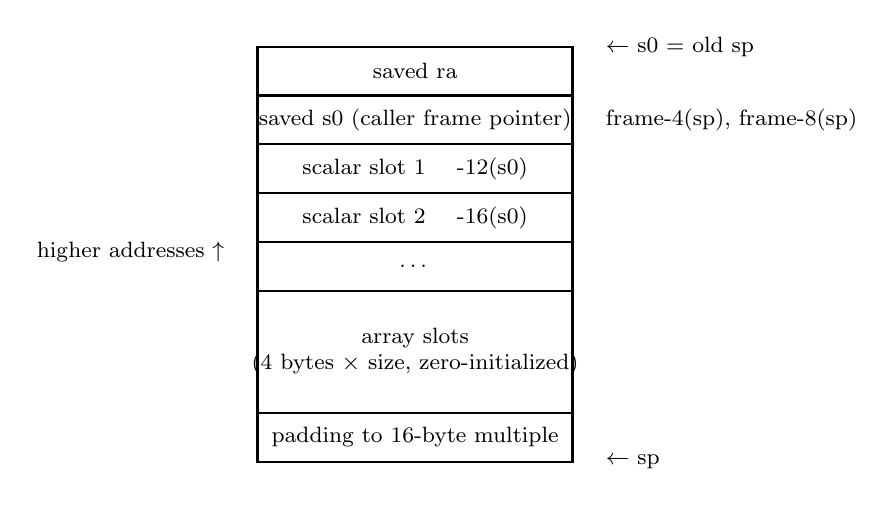
\begin{tikzpicture}[font=\footnotesize, yscale=0.62]
\draw[thick] (0,0) rectangle (4,1); \node at (2,0.5) {saved \code{ra}};
\draw[thick] (0,-1) rectangle (4,0); \node at (2,-0.5) {saved \code{s0} (caller frame pointer)};
\draw[thick] (0,-2) rectangle (4,-1); \node at (2,-1.5) {scalar slot 1 \quad \code{-12(s0)}};
\draw[thick] (0,-3) rectangle (4,-2); \node at (2,-2.5) {scalar slot 2 \quad \code{-16(s0)}};
\draw[thick] (0,-4) rectangle (4,-3); \node at (2,-3.5) {\ldots};
\draw[thick] (0,-6.5) rectangle (4,-4); \node[align=center] at (2,-5.25) {array slots\\(4 bytes $\times$ size, zero-initialized)};
\draw[thick] (0,-7.5) rectangle (4,-6.5); \node at (2,-7) {padding to 16-byte multiple};
\node[anchor=west] at (4.3,1) {$\leftarrow$ \code{s0} = old \code{sp}};
\node[anchor=west] at (4.3,-7.5) {$\leftarrow$ \code{sp}};
\node[anchor=west] at (4.3,-0.5) {\code{frame-4(sp)}, \code{frame-8(sp)}};
\node[anchor=east] at (-0.3,-3.2) {higher addresses $\uparrow$};
\end{tikzpicture}
\caption[Stack frame layout produced by the RISC-V back end for one function.]{Stack frame layout produced by the RISC-V back end for one function. Every IR name in the function receives a slot; no register allocation is performed.}
\label{fig:frame}
\end{figure}

Three semantic details are handled explicitly so that the assembly behaves exactly like the interpreter. Division and modulo are guarded by a branch that yields zero when the divisor is zero, because the hardware instructions would return $-1$ or the dividend. Comparisons are lowered to \code{slt}, \code{seqz}, \code{snez}, and \code{xori} sequences producing 0 or 1. Printing calls a built-in \code{print\_int} routine, emitted once per module, that converts a signed integer to decimal in a stack buffer and issues the Linux \code{write} system call; the program exits through the \code{exit} system call with \code{main}'s return value as status. Global variables are placed in a \code{.data} section and accessed with \code{la}/\code{lw}/\code{sw}. The generator also records, for every IR instruction, the range of assembly lines it produced, which the Assembly page uses for hover linking.

The simulator (\code{tests/riscv\_sim.py}, 213 lines) is a test oracle, not a general emulator. It parses exactly the instruction subset the generator emits, executes it with 32-bit wrap-around arithmetic, implements the two system calls, and captures standard output. A test compiles every benchmark under the best ordering and under no optimization, generates assembly, runs it in the simulator, and asserts that the printed integers and exit code equal the interpreter's. This closes the loop: an improvement measured on the IR is only reported if the lowered program still computes the same result.

\subsection{Web API and front end}

The FastAPI application (\code{compiler/web/app.py}, 495 lines, with Pydantic models in \code{api\_models.py}) exposes the endpoints in Table~\ref{tab:endpoints}. Every compile-like endpoint runs the front end and returns either the requested artefacts or a structured error record naming the phase (lexer, parser, semantic, IR generator, optimization, or runtime), the message, and the source line and column when known. Example names are validated against a strict pattern and resolved inside the benchmark directory only, so the file-serving endpoint cannot be used to read arbitrary files. The examples endpoint classifies each program as MiBench or PolyBench from its documentation comment and extracts that comment into a title and bullet points so the front end can present it.

\begin{table}[!htb]
\centering\small
\caption[HTTP endpoints exposed by the FastAPI server.]{HTTP endpoints exposed by the FastAPI server}
\label{tab:endpoints}
\begin{tabular}{L{4.3cm} L{8.9cm}}
\toprule
\textbf{Endpoint} & \textbf{Returns}\\
\midrule
\code{POST /api/compile} & tokens, serialized AST, symbols, IR records and text\\
\code{POST /api/optimize} & optimized IR, line diff, metrics, output, correctness, assembly\\
\code{POST /api/optimize-steps} & one stage per pass: IR text, diff against previous stage, size, cycles\\
\code{POST /api/assembly} & IR lines, assembly lines, IR-to-assembly line mapping\\
\code{POST /api/benchmark} & metrics for all 721 orderings and the baseline\\
\code{GET /api/examples} & name, description, and suite of each benchmark\\
\code{GET /api/examples/\{name\}} & source and structured documentation of one benchmark\\
\code{GET /}, \code{GET /legacy} & the React application; the zero-dependency legacy page\\
\bottomrule
\end{tabular}
\end{table}

The front end (\code{frontend/}, React 19 and TypeScript) is a single-page application with a sidebar and five pages. A typed API client mirrors the endpoint schemas. The shared editor component wraps CodeMirror 6 with a C language mode and a lint source that converts the server's error record into an underline at the reported position. A pipeline-rail component shows which stages of the pipeline a page exercises. The Playground compiles on load and offers tabs for tokens, a collapsible syntax tree, the symbol table, and the IR. The Optimization Lab presents the six passes as chips that can be dragged, or moved with the arrow keys for keyboard users, runs the ordering stage by stage, and shows the IR after any selected stage with removed lines struck through and added lines highlighted, together with the size and cycle deltas. The Assembly page shows IR and assembly side by side and highlights the assembly lines that correspond to the IR line under the cursor. The Phase Explorer runs all orderings and draws a scatter of size against cycles with the Pareto frontier highlighted and a bar chart of the ten smallest results; clicking a point reveals its ordering and metrics. The Reference page documents the passes, cost model, language, and pipeline. The build output is committed under \code{compiler/web/static/} so that the server works from a fresh clone without a JavaScript toolchain, and all fonts are bundled so the application works offline.

\subsection{Development history}

Table~\ref{tab:milestones} summarizes the development milestones as recorded in version control. The project was developed in two concentrated phases with a hardening step between them; 54 commits were made in total.

\begin{table}[!htb]
\centering\small
\caption[Development milestones recorded in version control.]{Development milestones recorded in version control}
\label{tab:milestones}
\begin{tabular}{L{2.4cm} L{10.8cm}}
\toprule
\textbf{Date} & \textbf{Milestone}\\
\midrule
11 Feb 2026 & Repository created; project proposal with the four-phase plan.\\
14 Apr 2026 & Design specification and implementation plan for the interactive tool. Lexer, parser, symbol table, IR, IR generator, interpreter, six passes, pass manager, metric collector, visualizer, eight MiBench-adapted benchmarks, command-line driver, single-file web UI, and first test suite delivered in one integration.\\
15--16 Apr 2026 & Hardening: fixed stale reuse in CSE, removed unsound boolean rewrites in AS, hardened the examples endpoint against path traversal, fixed the pass-interaction heatmap to use full-ordering data, added repository ignore rules.\\
5 Aug 2026 & Arrays added end to end: bracket tokens, AST nodes, symbol-table sizes, parsing, IR opcodes, IR generation, interpretation, array-aware passes, tests. Seven PolyBench-adapted array benchmarks added with documentation. Array cost model. Semantic analyzer, global variables, \code{for} loops, \code{else if}, short-circuit evaluation, shared error hierarchy, RISC-V RV32IM back end with simulator and 44 new tests. Web UI rebuilt as a React application with stepping, assembly, and explorer pages; examples grouped by suite. Documentation brought up to date.\\
6 Aug 2026 & Plot de-duplication for full-permutation datasets with regression tests; final benchmark plots regenerated.\\
\bottomrule
\end{tabular}
\end{table}

\section{Benchmark Dataset Description}

The dataset for this study is a suite of fifteen programs written in the supported C subset. Each is an adaptation of a kernel from a published benchmark suite, chosen so that the suite covers the control-flow and data-access patterns typical of embedded software (MiBench) and of numerical loop nests (PolyBench/C). The programs live in \code{compiler/benchmarks/programs/}, one file each, and every file begins with a documentation comment naming its source and the optimization opportunities it was designed to exercise. Table~\ref{tab:benchmarks} lists them with their baseline sizes.

\begin{table}[!htb]
\centering\small
\caption[The fifteen benchmark programs.]{The fifteen benchmark programs. Size is the static instruction count of the unoptimized IR; dynamic is the number of IR instructions executed by the interpreter.}
\label{tab:benchmarks}
\begin{tabular}{L{1.7cm} L{4.2cm} L{4.6cm} C{1.0cm} C{1.4cm}}
\toprule
\textbf{Program} & \textbf{Source kernel} & \textbf{Characteristic} & \textbf{Size} & \textbf{Dynamic}\\
\midrule
bitcount & MiBench automotive/bitcnts & loop, conditional, div/mod as shift/mask & 33 & 354\\
collatz & MiBench automotive patterns & unpredictable branching, mixed arithmetic & 42 & 4{,}712\\
factorial & MiBench basicmath & multiplication loop, planted dead code and CSE & 40 & 81\\
fibonacci & MiBench basicmath & iterative loop, rotating variable updates & 22 & 236\\
gcd & MiBench basicmath & Euclid's algorithm, modulo in loop & 21 & 45\\
isqrt & MiBench automotive/basicmath & Newton iteration, division-heavy & 50 & 347\\
power & MiBench security/blowfish & square-and-multiply modular exponentiation & 71 & 511\\
sha\_mix & MiBench security/sha & nested conditionals, modular mixing rounds & 106 & 2{,}522\\
jacobi1d & PolyBench stencils/jacobi-1d & array load/store, $i\pm1$ indexing, time steps & 76 & 1{,}064\\
jacobi2d & PolyBench stencils/jacobi-2d & flattened 2-D grid, five-point stencil & 144 & 2{,}787\\
gemm & PolyBench blas/gemm & triple loop, multiply-accumulate into array & 164 & 3{,}081\\
2mm & PolyBench kernels/2mm & two chained matrix products, five live arrays & 252 & 5{,}259\\
atax & PolyBench kernels/atax & two reductions sharing an intermediate array & 101 & 1{,}448\\
bicg & PolyBench kernels/bicg & two accumulators from one shared load & 94 & 1{,}283\\
gesummv & PolyBench blas/gesummv & two matrix-vector products plus scalar combine & 106 & 1{,}487\\
\bottomrule
\end{tabular}
\end{table}

\textbf{Adaptation rules.} The source language has no bitwise operators, no floating point, no two-dimensional arrays, and no input. The kernels were adapted under four rules. Bit operations are expressed with division and modulo by two, which are semantically identical for non-negative operands (\code{bitcount}). Floating-point kernels are made integer, with divisions used where the original averaged (\code{jacobi1d}, \code{jacobi2d}). Two-dimensional arrays are flattened to one dimension with explicit row-major index arithmetic \code{a[i * n + j]}, which is faithful to how a C compiler lays them out and which produces exactly the repeated index expressions that common subexpression elimination and strength reduction target. Inputs are fixed to small constant problem sizes (matrices of $4\times4$ or $5\times5$, vectors of 5 or 8 elements, a handful of time steps) initialized by simple arithmetic formulas, and results are printed so that the interpreter's output is a complete witness of the computation; every printed value participates in a checksum that is also returned. Listing~\ref{lst:jacobi1d} shows one adapted kernel in full.

\begin{lstlisting}[language=CSubset, caption={The \code{jacobi1d} benchmark, adapted from PolyBench/C stencils/jacobi-1d. Two buffers alternate over four time steps; each interior element becomes the integer mean of itself and its two neighbours.}, label={lst:jacobi1d}]
int main() {
    int n = 8;
    int steps = 4;
    int a[8];
    int b[8];

    int i = 0;
    while (i < n) {
        a[i] = (i * i) % 7 + 1;
        i = i + 1;
    }

    int t = 0;
    while (t < steps) {
        i = 1;
        while (i < n - 1) {
            b[i] = (a[i - 1] + a[i] + a[i + 1]) / 3;
            i = i + 1;
        }
        i = 1;
        while (i < n - 1) {
            a[i] = b[i];
            i = i + 1;
        }
        t = t + 1;
    }

    i = 0;
    while (i < n) {
        print(a[i]);
        i = i + 1;
    }
    return a[n / 2];
}
\end{lstlisting}

\textbf{Coverage.} The eight MiBench-derived programs are scalar: they exercise function calls, loops with data-dependent trip counts, conditionals, and integer arithmetic including expensive division and modulo. Two of them (\code{factorial} and \code{sha\_mix}) contain planted dead code and repeated subexpressions so that every pass has visible work on at least one program. The seven PolyBench-derived programs are array-based: they exercise array loads and stores, repeated affine index arithmetic, and deep loop nests, and they contain no planted opportunities; whatever the passes find in them is what a compiler would find in real numerical code. The two groups behave measurably differently under optimization, as Chapter 5 shows.

\section{Tools and Technologies used for Implementation}

\begin{itemize}
  \item \textbf{Python 3.12.} The compiler, interpreter, passes, back end, benchmark driver, and web server are written in Python with type annotations and dataclasses throughout. Python was chosen for readability, since the code is meant to be read by students, and for speed of development; its performance is more than sufficient, since the full 10{,}815-compilation benchmark runs in about 24 seconds.
  \item \textbf{FastAPI 0.141, Uvicorn 0.52, Pydantic 2.} The web server. FastAPI provides typed request and response models, automatic validation, and an interactive API description; Uvicorn is the ASGI server. The server serves both the JSON API and the static front end from one process.
  \item \textbf{React 19, TypeScript 6, Vite 8.} The front end. React components map naturally onto the pages and shared widgets; TypeScript's types mirror the Pydantic models so that API changes are caught at build time; Vite builds the application into the static directory served by FastAPI.
  \item \textbf{CodeMirror 6.} The source editor, with the C language mode for highlighting and the lint extension for underlining compiler errors at their reported positions.
  \item \textbf{Chart.js 4 with react-chartjs-2.} Interactive scatter and bar charts in the Phase Explorer, with hover tooltips and click-to-select.
  \item \textbf{matplotlib 3.11 and NumPy 1.26.} Publication-quality static plots from the benchmark driver, rendered headlessly with the Agg back end.
  \item \textbf{pytest 9.} The test framework; 185 test cases in three modules, including parametrized end-to-end tests over all benchmarks and all orderings.
  \item \textbf{RISC-V GNU toolchain and QEMU (optional).} The generated assembly is written for \code{riscv64-linux-gnu-gcc -march=rv32im -mabi=ilp32} and \code{qemu-riscv32}; they are not required because the bundled simulator validates the assembly in the test suite.
  \item \textbf{Git and GitHub.} Version control and collaboration; the repository history is summarized in Table~\ref{tab:milestones}.
  \item \textbf{Visual Studio Code, Linux Mint 22.2, Windows.} Development environments. The system runs unchanged on both operating systems.
  \item \textbf{Bundled fonts: Inter, JetBrains Mono, Space Grotesk.} Packaged with the front end so the application has no network dependency.
\end{itemize}
